\section{Language Models - Tokenizer}\label{sec:b}


\epigraph{A picture is worth a thousand words, and a word is worth around 0.75 tokens.}{\textit{Unkown, 2024}}

Today the \glspl{LM}, whether large or small, can understand and produce human language (to some extent), but we know that the way that these models process the text differs from how we do it. A \gls{LM}, before it can start to work with any text, needs a way to break down and translate that text into a form of information that it can process, namely, numbers. This is where the \emph{tokenizer} comes in.

In this sections we briefly introduce the concept of \textit{token}, \textit{tokenization} and \textit{tokenizer} and how they work in a \gls{LM}. Later we describe an issue that the \gls{MLTB} (and the POKT Network) faces when trying to interact with unknown \glspl{LM} and propose a requirement for the deployment of models that will solve it.

\subsection{From string to token}\label{subsec:b1}

Formally, the \emph{tokenization} is the process of representing text in smaller meaningful lexical units, called \emph{tokens}. Meaning, breaking it apart in a way that is useful and information is preserved, and assigning each part an unique number. There are three popular ways to do the same, which are:
\begin{itemize}
    \item \textbf{Word Tokenization :} This is the simplest form of tokenization, where each word is considered a token. 
    \item \textbf{Sub-Word Tokenization :} Breaking words into subwords and treat each part as tokens.
    \item \textbf{Character Tokenization :} A very naïve tokenization that considers each character as a token. 
\end{itemize}

As always, there is a trade-off between the different approaches, in this case the granularity of the tokens (how many you need to decompose a text) and the number of tokens (how many unique tokens you have). That is, while word tokenization has low granularity and high token count, character tokenization has high granularity and low token count.

Nowadays, the most popular tokenization method is subword tokenization, which is a compromise between word and character tokenization. 
Tokenizers (advanced ones at least) are standalone machine learning techniques~\cite{kudo_sentencepiece_2018,kudo_subword_2018,sennrich_neural_2016} whose output is dictionary that assigns numbers (tokens) to different strings. It is important to note that prior to training a model, tokenizers must be trained on texts that is representative of the training set (ideally the tokenizer texts should not be part of the training set). So, when training a \gls{LM} for technical english text, the tokenizer should be trained on technical english words, and as a result you should have an effective description of the language to use. For example such a tokenizer might assign a single token to word that repeats to much in technical english, like "therefore", but have to use 2 tokens to represent other common english words such as "puppy" (using "pup" and "py" maybe), because they are rare in technical english.

As we said, the tokenizer is the one in charge of carrying out the tokenization process, which consists (in a nutshell) of a dictionary that contains pairs of tokens and their numerical representation. This numerical representation is the actual data that is analyzed by the \gls{LM} and for this reason, a direct relationship is established between a \gls{LM} and its tokenizer.


\subsubsection*{Tokenizers in Language Models Evaluations}

This relationship between a \gls{LM} and tokenizer is crucial when evaluating the performance of a \gls{LM}, since one of the main techniques for evaluating a language \gls{LM} is through the calculation of the probability of occurrence of a sequence of tokens that is conditioned by an initial sequence of tokens. In other words, the probability of following a sentence with a given set of words, when some initial words (context) are provided. 
In terms of \texttt{lm-eval-harness}~\cite{biderman_lessons_2024} these two sequences are also called \texttt{context} and \texttt{continuation}, as shown in Figure \ref{fig:loglikelihood_example}.

\begin{figure}[h]
    \centering
    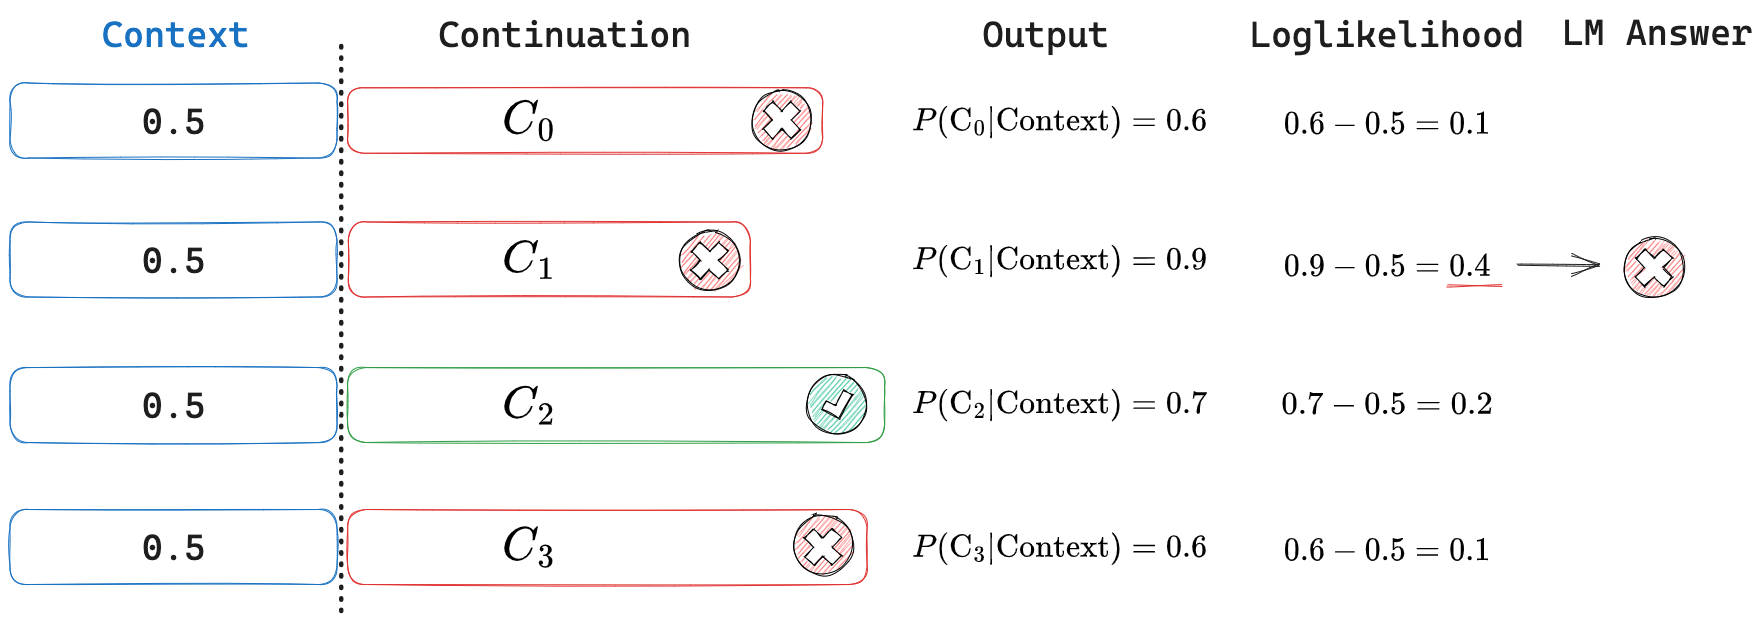
\includegraphics[width=\textwidth]{img/loglikelihood_example.png}
    \caption{Example of \texttt{context}, \texttt{continuation} token sequences and evaluation result. The green segment in \texttt{continuation} represents correct segment (ground truth), the \emph{Loglikelihood} column represents the segment of higher probability (assigned by the \gls{LM}), and finally the \emph{LM Anwer} correspond to the result of the evaluation example. In this case, $C_2$ should be the higger probability, nevertheless the \gls{LM} returns $C_1$ with higher probability.}
    \label{fig:loglikelihood_example}
\end{figure}

Without going into the mathematical details, and following the Figure \ref{fig:loglikelihood_example}, the concatenation of the \texttt{context} and \texttt{continuation} tokens is sent to the \glspl{LM}, and from their returns it can be computed the probability of occurrence of the entire phrase, detailed token by token. 
The \gls{LM} is considered to respond correctly when the probability of occurrence of the correct \texttt{continuation} is the highest with respect to the other continuations. That is, in terms of the Figure \ref{fig:loglikelihood_example}, the \gls{LM} responds incorrectly, since $C_2$ should have been the \texttt{continuation} with the highest probability, but the \gls{LM} returns a higher probability for $C_1$. 


\subsection{On the lack of knowledge of the tokenizer}\label{subsec:b2}

Not knowing the tokenizer of a model might be irrelevant when we are only interested in interacting with a model. As long as the \gls{API} accepts plain text, we can use the served \gls{LM}. While this is true, it restricts the versatility of solutions that we can construct around the POKT network. Specifically it poses difficulties in the following aspects:

\subsubsection*{Decentralized Evaluations}

As previously detailed, the \gls{LM} receives the concatenation of the \texttt{context} and \texttt{continuation} token sequences, and then locally separates the \texttt{context} and \texttt{continuation} probabilities. 
However, in a decentralized environment, such as that proposed by \gls{MLTB}, if you do not have access to the tokenizer, it is not possible to separate the \texttt{context} and \texttt{continuation} probabilities. 
While the plain text of the concatenation of context and \texttt{continuation} could be sent, we could not directly determine which part of the text belongs to the \texttt{context} and which part belongs to the continuation, thus preventing the evaluation of the model. 
Although one could try to reconstruct the \texttt{context} and \texttt{continuation} phrase from the concatenation of tokens, this is not a trivial task, since the tokenizer could have tokenized differently than the original text was tokenized \cite{biderman_lessons_2024}. 

\subsubsection*{Price and Query Optimization}

The gateways deployed in the POKT Network will probably want to be able to infer the price of a call prior sending it to a \gls{LM}-Node. While currently we do not count tokens, it is expected that the price of a \gls{LM} \gls{RPC} will be modulated by the number of tokens being processed (in some way or to some extent at least). Knowing the tokenizer nature will become a necessity to estimate and optimize the \gls{RPC} calls.

\subsubsection*{Model Verification}

Given the \gls{LM}-\emph{Tokenizer} relationship, knowing the tokenizer of a model already let us know something about it. A tokenizer can be used in many models, but a model can use a single tokenizer, this way we reduce the search space of models if we know its tokenizer. Also, if the tokenizer changes at some point, we can be sure that the served model changed.

Another important fact is that we must remain open to model verification techniques. For example, one of these techniques is called \emph{watermarking}~\cite{kirchenbauer2023watermark} and works by detecting the presence of probabilities of certain \emph{tokens} in the produced text.


\subsection{Proposed solution}\label{subsec:b3}

Faced with this situation, there are three other plausible solutions (at least for the \gls{MLTB}). 

The first solution would be to send, in addition to each complete sentence, only the \texttt{context} text. 
This would then allow us to remove those corresponding to the \texttt{context} from each of the complete sentences and continue with the evaluation of the model. 
The disadvantage of this solution is that $N+1$ calls would be made to the model, where $N$ is the number of complete sentences to evaluate, resulting in a higher cost. 
Furthermore, in the case of evaluations that contemplate the use of conversational models (such as the case of chat), this solution would not be applicable, since internally these models through its toke add special tokens to indicate the beginning and end of a message in a conversation, just as they usually have a text to condition the model's response, called system prompt. 

The second solution would be online tokenization, calling for example an endpoint \emph{tokenize} (in a custom \gls{API}). 
This situation would face similar problems, as currently discussed in the community \footnote{\url{https://github.com/huggingface/text-generation-inference/issues/1706}}. 

The third solution would involve sending the complete tokenizer associated with an node address. 
This was detailed in two PRs \footnote{\url{https://github.com/EleutherAI/lm-evaluation-harness/pull/1794}} \footnote{\url{https://github.com/vllm-project/vllm/pull/2643}} in both the \gls{LMEH} repository and the vLLM repository, a popular \gls{LM} inference engine. 
The main advantage of this solution is that the issues of the first and second solutions are avoided. 
Additionally, as previously detailed, the tokenizer is tied to the model. 
Therefore we can generate a hash of the tokenizer that sends us an address, save it in a database and then verify that the hash of the tokenizer that is sent at the beginning of a session is equal to the hash stored in the database. 
If for some reason the hash does not match, it is an unequivocal indication that the \gls{LM} behind the endpoint is not the same, it has changed, therefore the previous results are not valid, metrics are eliminated from the leaderboard, and that address has to be re-evaluated. 

From these three solutions we argue that the third one (having access to the full tokenizer) is the best to implement in the POKT Network. This solution is based on solutions that already being implemented in the \gls{LM} community and provide us with the largest versatility for future developments.